% created on 27/11/2020
% @author : ebazan

\chapter{Perceptual Object Segmentation Model}

\section*{Résumé}
\noindent 

\section*{Abstract}
\noindent 

\section{Introduction}
In Chapters \ref{ch:spectral_image_decomposition} and \ref{ch:complex_spectral_image_decomposition} we have introduced the theoretical aspects of gabor filters and their use in a complex color space. Using the family of filters as a measurement tool, we created a feature space that exploits the color and texture information of the images and the relationship between them. This feature space can be seen as the complex spectral decomposition of an image.

In this chapter we propose a workflow to use in the image segmentation task. We have seen that it is possible to obtain unsupervised segmentation using some clustering method on the proposed feature space (see section). However, clustering methods have the limitation of needing some kind of a priori information, for example the number of clusters or objects in the image. The objective of the proposed framework is to obtain a coherent segmentation of the image using the fewest possible parameters.

The present framework obtains the segmentation of an image from the perceptual gradient of the objects. The overall idea of our framework can be seen in the diagram of figure \ref{fig:pipeline_gabor_image_segmentation}. First, we represent the image as a graph (which can be pixel-based or region-based). Next, we calculate the graph's edge's weight using the concept of optimal transport through the EMD (see section \ref{subsec:EMD}), which is a measure that reflects the true distance between two distributions. Finally, the representation of the image as an edge-weighted graph allows to straightforward apply various graph-based segmentation techniques or, to recover the perceptual boundaries of the image in the form of a gradient image, on which we can apply some gradient-based segmentation techniques.


\begin{figure}[!ht]
	\centering
	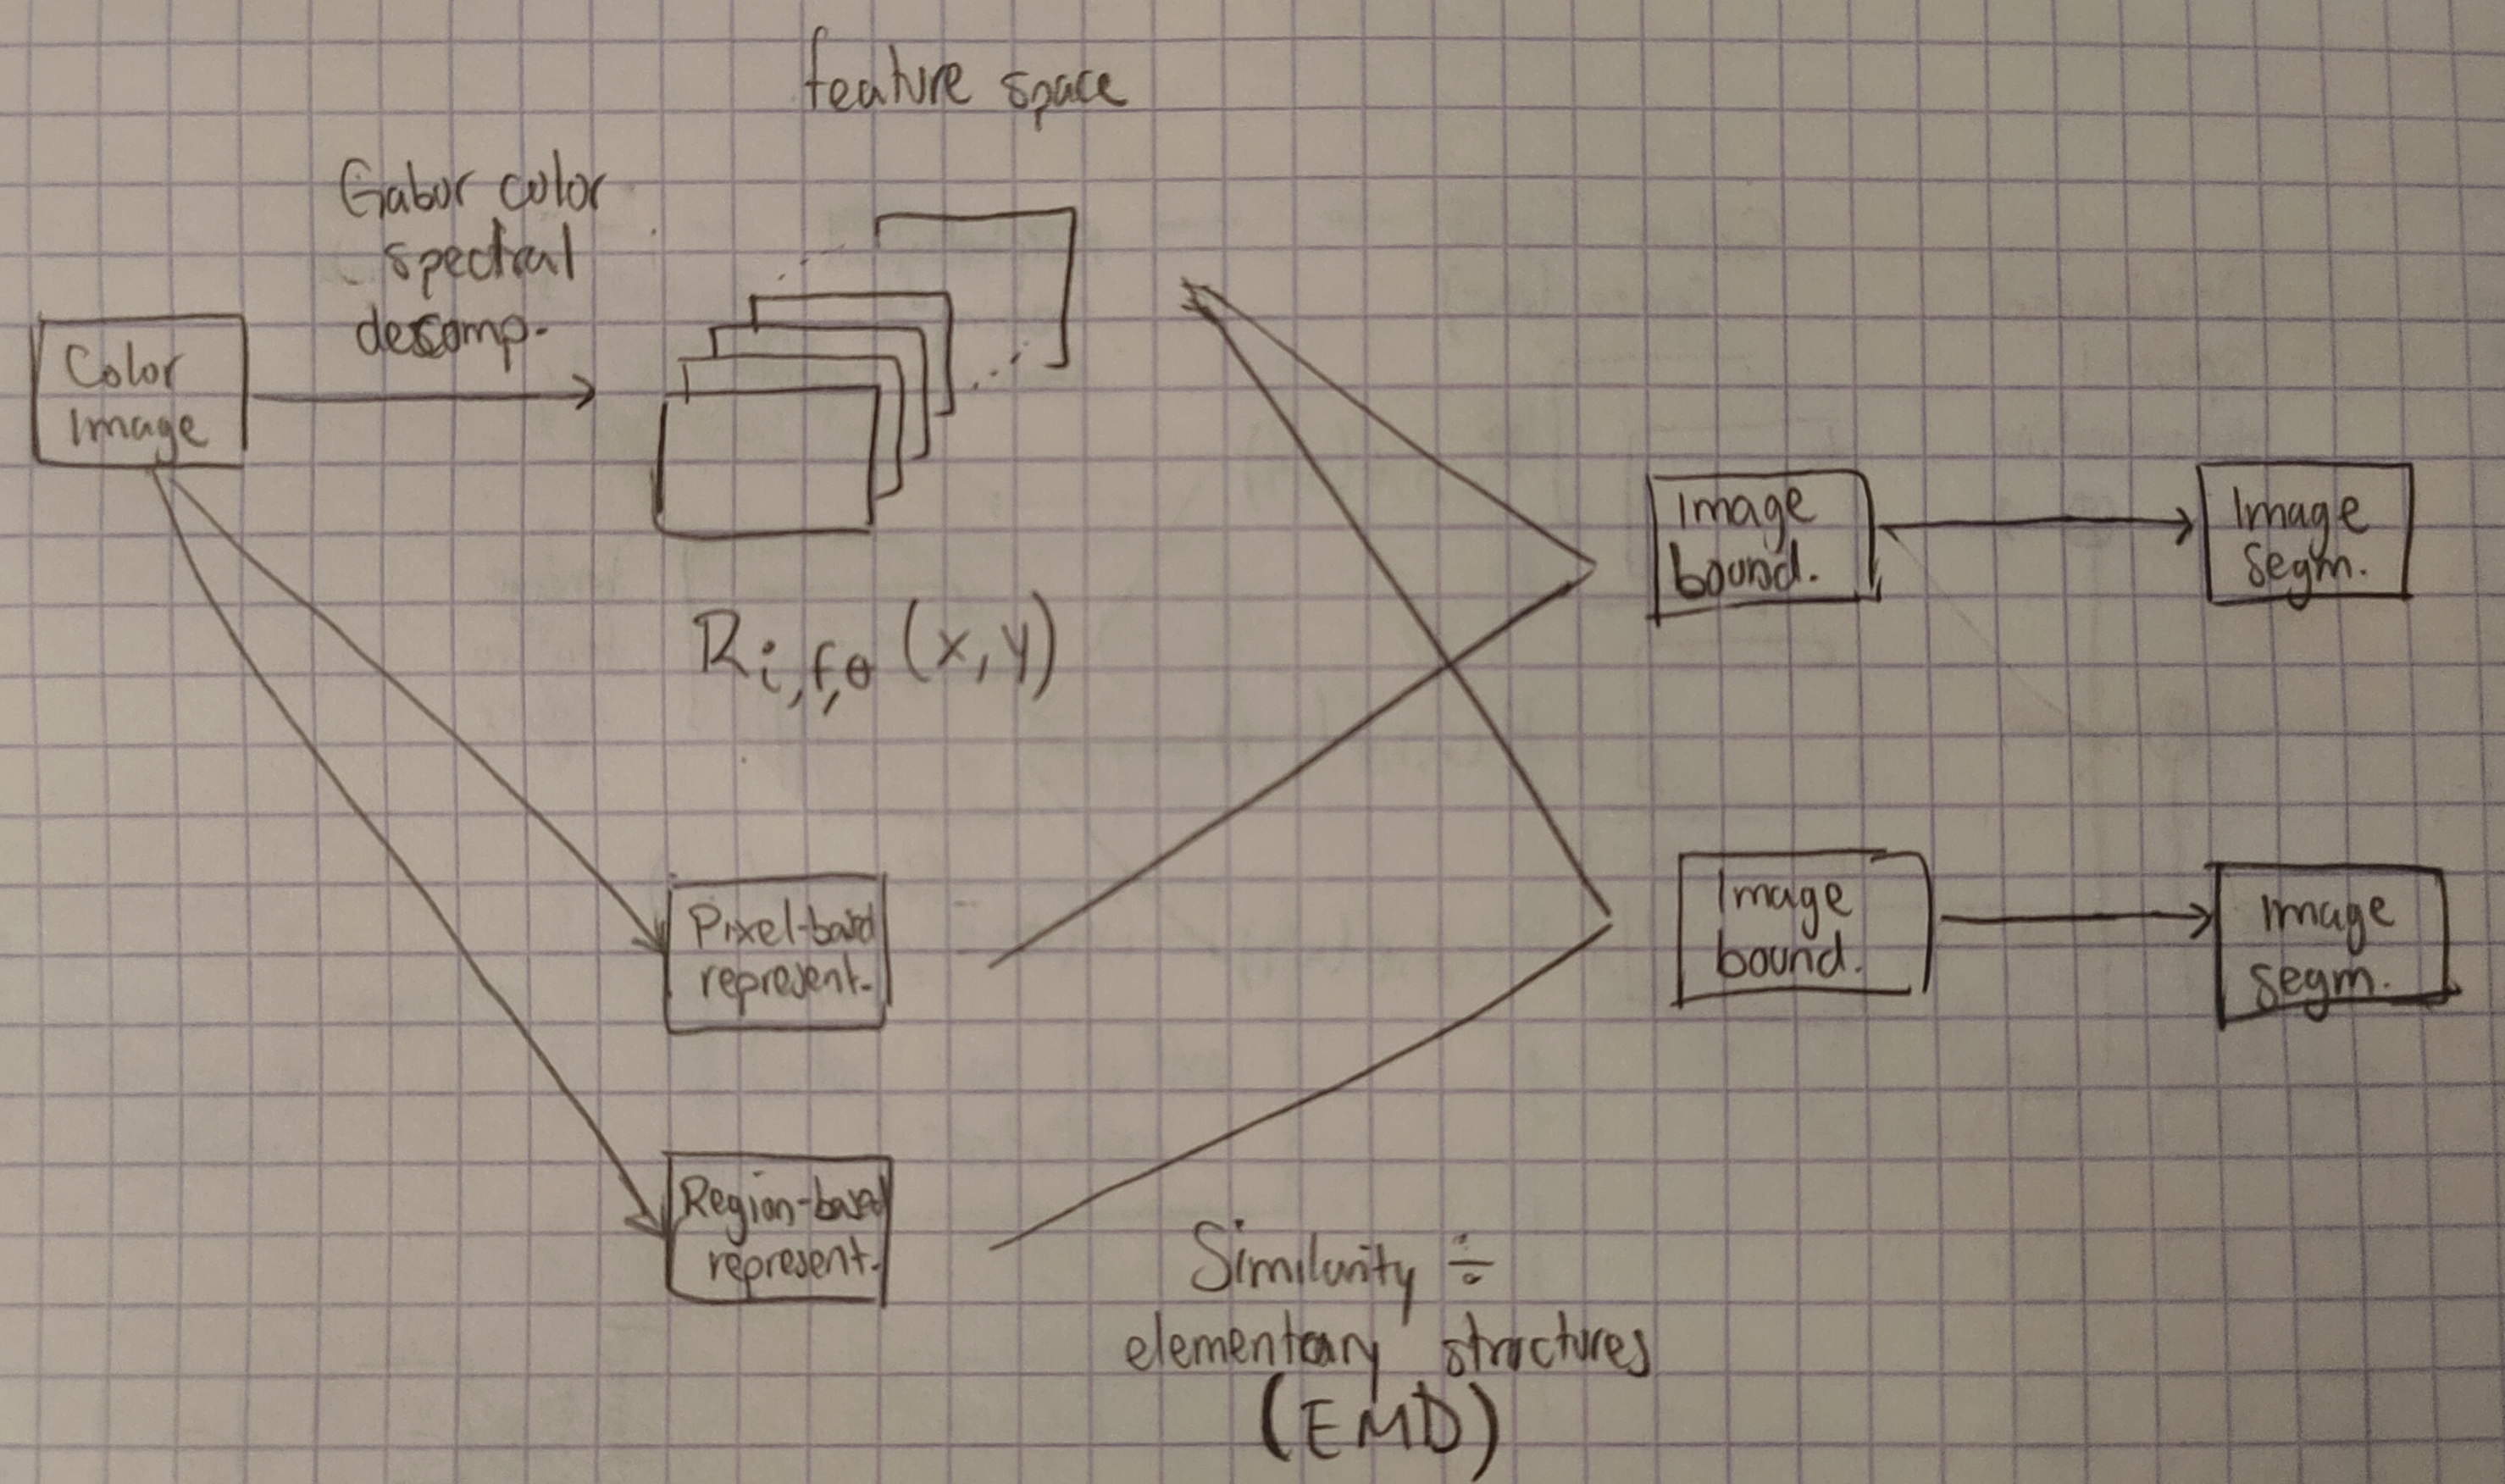
\includegraphics[width=\textwidth]{image_segment_gabor_features}
	\caption{General pipeline for extraction of perceptual imagen boundaties and unsupervised image segmentation.}\label{fig:pipeline_gabor_image_segmentation}
\end{figure}

\section{Related work}
Edge detection is a fundamental problem of computer vision that has been intensively studied since the early 1970s \citep{Hueckel:JACM:1971, Fram.Deutsch:TC:1975}. The main idea behind traditional approaches to contour extraction is to model edges as discontinuities in the brightness channel of an image. This idea gave way to the creation of mask-based operators such as Sobel \citep{Maitre:Book:2003}, Roberts \citep{Roberts:Thesis:1963}, Gradient \citep{Maitre:Book:2003} and Prewitt \citep{Prewitt:PPP:1970}, which quantify the presence of an edge through the convolution of a gray level image with local derivative filters. Other techniques, such as Marr and Hildreth \citep{Marr.Hildreth:PRS:1980}, define edges as the zero crossings of the Laplacian of a Gaussian (LoG). Within traditional methods, the Canny \citep{Canny:PAMI:1986} operator is one of the most popular approaches to this day. This operator follows the same principle of operation of the previous methods, adding a non-maximum suppression stage and a hysteresis thresholding.

Despite their efficiency in controlled environments or in synthetic images, traditional methods suffer when it comes to identifying contours in natural images. The edges of natural images can be present at different scales, and the colors and textures of the scene can generate edges that are perceptually significant to the human eye. Ideally, a contour detection method is intended to simultaneously exploit the brightness, color and texture properties of an image in such a way that it can handle the boundary perimeters defined by the brightness steps and the regions with constant color and / or texture.

One of the relatively recent strategies for identifying perceptual contours is to use the local energy response of an image. The principle of operation is simple: generate features from the responses of an image produced by a family of filters at different scales and orientations. The idea has been exploited from different points of view. For example, the use of the  Difference of Gaussians (DoG) and its HIlbert transform \citep{Morrone.Owens:PR:1987, Morrone.Burr.ea:RSL:1988} for the generation of a family of filters. Inspired by Gabor's work, this group of filters comply with the Parseval principle; in addition to generating an exact quadrature pair (even and odd symmetry cells).

The \textit{Probability-of-boundary} (Pb) detector \citep{Malik.Belongie.ea:IJCV:2001} is one of the major exponents of the use of a filter bank formed by the DoG and its Hilbert transform. The contour detector only uses the brightness and texture information to obtain the Pb. The brightness information is processed following the intervening contour framework \citep{Leung.Malik:ECCV:1998} which consists in obtaining the quadrature energy of the image, also called oriented energy (OE). The texture information is analyzed using so-called textons \citep{Malik.Belongie.ea:ICCV:1999}. Since each cue (brightness and texture) has a domain of applicability, hence different units of magnitude, they introduce a gating operator based on the texturedness of a neighborhood at a pixel. The operator give as a result a local measure which indicates how much two nearby pixels are to belong to the same region. Later in that work, they use spectral graph theory (normalized cut algorithm \citep{JianboShi.Malik:PAMI:2000}) to segment the image into regions of coherent texture and brightness.

This contemporary method, developed by the UC Berkeley research group, was the basis for many other techniques for contour detection and segmentation of natural images widely used today. Most of these works bring substantial improvements to the Pb detector. For example, the seminal papers \citep{Martin.Fowlkes.ea:NIPS:2002} and \citep{Martin.Fowlkes.ea:PAMI:2004} bring together previous works related to Pb and obtain a feature space of four image characteristics: localized OE, Brightness Gradient (BG), Color Gradient (CG) and localized Texture Gradient (TG). To cope with the problem of the difference in units of magnitude of the cues, they use a logistic regression classifier to combine oriented energy, brightness, color and texture. The proposed supervised method optimizes the weights of each feature formulating it as a two-class classification problem, where they learn the rules for combining cues from the groundtruth data of the Berkeley Segmentation Dataset (BSDS) \citep{Martin.Fowlkes.ea:ICCV:2001}.

On the other hand, \cite{Ren:ECCV:2008} showed that the Pb detector improves when using features of the image calculated at different scales. However, a better version of the Pb detector, which has dominated the state of the art scores for several years, is obtained by combining local and global contours \citep{Maire.Arbelaez.ea:CVPR:2008}. The local contours are represented by the multiscale oriented signal mPb, while the global contours are represented by the oriented signal from the spectral partition sPb. The final detector that combines both signals is the globalized Probability-of-boundary gPb, which learns the weights of the local and global part by means of an ascending gradient, taking as reference the BSDS evaluation score.

The Berkeley research group laid the foundation for contour detection and natural image segmentation, providing tools for quantitative comparison of methods. However, there are other methods in the literature that use different strategies to calculate image features and detect contours. Such methods can use fully supervised approaches, avoiding the careful hand-drawing of texture and gloss gradients. However, we can also find semi-supervised methods that replace the Pb detector to later apply a preprocessing chain similar to that applied in the Berkeley group methods.

The Berkeley research group laid the foundation for contour detection and natural image segmentation, providing the database and tools for the comparison and quantitative evaluation of the different approaches. Furthermore, Pb has motivated the development of state-of-the-art methods that use totally different strategies to obtain image features and contour detection. Such methods can use fully supervised approaches, avoiding careful filter design, computation of texture and brightness gradients, and hand-crafted features. We can also find semi-supervised methods, which generally replace the Pb detector with a supervised detector to later apply a preprocessing chain similar to that applied in the Berkeley group methods to refine the detection.

The set of the most popular supervised methods for contour detection, led by researchers from the University of Pasadena California and colleagues, is based on the calculation of features on channels of integrals of the image \citep{Dollar.Tu.ea:BMVC:2009}. Some examples of these integral channels are: image color and gray channels, image responses to linear filters (e.g. Gabor filters, DoG), non-linear image transformations (e.g. Canny edges, gradient magnitude, hysteresis threshold), among others. The calculation of features on the integral channels follow the object detection framework of \cite{Viola.Jones:IJCV:2004}, obtaining first-order and higher-order features such as Haar-like features. Following this principle, a pool of features is obtained by randomly choosing both the integral channel and a rectangle on which the features are calculated, which allows the acceleration of the computation of features and the application of boosting techniques for learning.

Some of the supervised edge detectors that use the integral channel features as input are the Boosted Energy Learning (BEL) \citep{Dollar.ZhuowenTu.ea:CVPR:2006}, which attempts to learn an edge classifier in the form of a probabilistic boosting tree from the thousands of simple features calculated in image patches. On the other hand, Sketch tokens \citep{Lim.Zitnick.ea:CVPR:2013} uses the same features as input to a random forest classifier. The peculiarity of this second method is that the classes of the classifier are the so-called sketch tokens; mid-level information patches that represent complex shapes such as joints, corners, vertical and horizontal edges, etc., calculated from the contours of the groundtruth. The Structural Edge (SE) detector \citep{Dollar.Zitnick:ICCV:2013} and its different versions \citep{Dollar.Zitnick:PAMI:2015} take these strategies to another level, learning not only the integral input features but also the output space, using structured-output decision forests. The Oriented Edge Forest (OEF) detector \citep{Hallman.Fowlkes:CVPR:2015} outperforms existing supervised methods by using a decision forest that analyzes local patches and outputs probability distributions over the space of oriented edges passing through the patch. Finally, the detector based on a Deep Neural Network (DeepNet) architecture \citep{Kivinen.Williams.ea:PMLR:2014}, is a fully supervised method that does not use the integral features framework, instead, it calculates complex-cell like covariance features from multiple scales and semantic levels, which depend on the squared response of a filter to the input image.

Another group of approaches to contour detection are those based on local sparse coding. Such techniques are said semi-supervised because they contain two main stages, one unsupervised and the other supervised. The first stage consists of obtaining a generic representation (without information of the contours) from the information of the image in an unsupervised way. The second stage consists of transforming the sparse representation of the image into a specific labeling task, where in the case of contours detection is a two-classes supervised problem, which that lables the pixels as contour or no contour. Some renowned works under this approach are the detector proposed by \cite{Mairal.Leordeanu.ea:ECCV:2008} and the Sparse Code Gradients (SCG) detector \citep{Ren.Bo:NIPS:2012}. Both works use K-SVD as a dictionary learning algorithm and Orthogonal Matching Pursuit for efficient optimization and sparse coding of each pixel. At the end of the process, they use SVM as linear classifier on the feature vectors resulting from the reconstruction error with each dictionary for pixel classification. The main difference between these detectors is that the SCG adopts the same scheme as the Pb detector, replacing the brightness, color and texture gradients with sparse code gradients. Finally, the Sparse Code Transfer (SCT) detector \citep{Maire.Yu.ea:ACCV:2014} improves on the detector of \cite{Mairal.Leordeanu.ea:ECCV:2008} using a greater number of dictionaries at different scales and layers in addition to the multipath sparse coding technique, which rectifies the initial sparse codes to reconstruct the contours with an extra transfer dictionary. The main disadvantage of these semi-supervised methods is the computational time of both processes, dictionary calculation and learning.

There is a fine line between the contour detection and image segmentation. In this sense, the Pb contour detector has also had an influence on image segmentation. The Ultrametric Contour Maps (UCM) \citep{Arbelaez.Maire.ea:PR:2009} uses the gPb to define a measure of dissimilarity (ultrametric distance) between pairs of adjacent regions defined by a hierarchical segmentation operator (HSO). This technique is refined by adding a supplementary preprocessing stage using the oriented watershed transform (OWT), giving rise to the gPb-owt-ucm hierarchical segmentation method \citep{Arbelaez.Maire.ea:PR:2009}. The extensive qualitative and quantitative comparison of these techniques can be consulted in \citep{Arbelaez.Maire.ea:PAMI:2011}.

The Pb contour detector has driven (directly or indirectly) 50 years of research work around the detection of perceptual contours in natural images their segmentation. Like the Canny operator, the Pb operator has become the reference work. The importance of this method is that it provides a good basis that takes into account the principles of human perception, using operators that have a physical sense.


\begin{table}[]
\begin{tabular}{c|c|c|c}
\textbf{Edge detector} & \textbf{Input features}                                                                           & \textbf{Main approach}                                           & \textbf{\begin{tabular}[c]{@{}c@{}}Segmentation \\ technique\end{tabular}} \\ \hline
Pb                      & BG, TG                                                                                            & Gradients dissimilarity                                          & Normalized cuts                                                            \\
PMI                     & LUV color channels                                                                                & Pixel mutual information                                         & -                                                                          \\ \hline
SCG                     & \begin{tabular}[c]{@{}c@{}}Gray, color, and \\ depth channels\end{tabular}                        & \begin{tabular}[c]{@{}c@{}}Sparse coding\\ +\\ SVM\end{tabular}  & -                                                                          \\
SCT                     & RGB color channels                                                                                & \begin{tabular}[c]{@{}c@{}}Sparse coding\\  +\\ SVM\end{tabular} & -                                                                          \\ \hline
$\widehat{\text{Pb}}$   & BG, TG                                                                                            & Logistic regression                                              & Normalized cuts                                                            \\
gPb                     & $\widehat{\text{OE}}$, BG, CG, $\widehat{\text{TG}}$                                              & Logistic regression                                              & UCM + OWT                                                                  \\
BEL                     & Integral channel features                                                                         & Gradient boosting                                                & -                                                                          \\
Sketch tokens           & Integral channel features                                                                         & Random forest                                                    & -                                                                          \\
SE                      & Integral channel features                                                                         & Random forest                                                    & -                                                                          \\
OEF                     & Integral channel features                                                                         & Random forest                                                    & -                                                                          \\
DeepNet                  & Covariance-like features                                                                          & Deep NN                                                          & -                                                                          \\
ISCRA                   & \begin{tabular}[c]{@{}c@{}}BG, CG, TG, SIFT,\\  shape features, \\ boundary features\end{tabular} & Cascading classifier                                             & Region merging                                                             \\
COB                     & $\widehat{\text{OE}}$, BG, CG, $\widehat{\text{TG}}$                                              & Convolutional NN                                                 & -                                                                       
\end{tabular}
\end{table}

\section{Image as a graph}

Graphs are historical mathematical structures that have been applied to almost all fields of engineering. Historically, Euler made use of these structures to solve a problem related to the optimal crossing of people across bridges. The success of these structures in fields such as electricity and chemistry, contributed to the creation of a standard nomenclature, giving way to the Graph theory.

Fundamentally, a graph is an useful structure for modeling pairwise relations between objects. In the field of image processing we can find several approaches that make use of graphs. Generally these methods solve a minimization problem. For example, the \textit{minimun spanning tree} approach that aims to find for each pair of nodes, the path with the least weight edges. On the other hand, the \textit{max-flow min-cut} approach aims to maximize flow with the minimum number of cuts in the graph. Both strategies have been successfully applied to the image segmentation problem. Another application example involves the algebraic theory of graphs that studies the spectrum of matrices that represent graphs.



\subsection{Graph notations and definitions}

In this section we introduce some important definitions that will be used throughout the chapter related to graphs and some related structures.

\begin{definition}[Graph]
	A graph $\mathcal{G}$ is defined by the finite sets $(\mathsf{V}, \mathsf{E})$ in which $\mathsf{E} \subset \mathsf{V} \times \mathsf{V}$. The elements of $\mathsf{v} \in \mathsf{V}$ are called \textit{vertices} and the elements of $\mathsf{e} \in \mathsf{E}$ are called edges. Since the edges are a subset of two nodes, we can write them as $\mathsf{e}_{i,j}$ or $\{i,j\} \forall i, j \in V$.
\end{definition}

\begin{definition}[Neighborhood]

\end{definition}

\begin{definition}[Subgraph]

\end{definition}

\begin{definition}[Edge-weighted graph]

\end{definition}

\begin{definition}[Node-weighted graph]

\end{definition}

\begin{definition}[Adjacency]

\end{definition}

\begin{definition}[Adjacency matrix]

\end{definition}



\subsection{Pixel-based representation}


\subsection{Region-based representation}
The term \textit{superpixels} was introduced by (cite Ren and Malik) in 2013. The term superpixels emerge as an oversegmentation process. The motivation lies in the affirmation that pixels are not natural entities, they are consequence of the discrete representation of an image and also that the number of pixels is to high (even in moderate resolutions) making the optimization at pixel level difficult. The superpixels are local coherent and preserve most of the stucture necessary for the segmentation.  

The superpixels technique comes from the oversegmentation techniques; to make the difference between them we can consider the following requeriments:
\begin{enumerate}
 \item Partition. Superpixels should define a partition of the image. They should be disjoint and assign a label to every pixel.
 \item Connectivity. Superpixels represents a connected set of pixels.
 \item Boundary Adherence. Superpixels must preserve image bundaries.
 \item Compactness, Regularity and Smoothness. Superpixels should be compact (closed and bounded), placed regulary and exibit smooth boundaries.
 \item Efficiency. Shuold be generated efficiently
 \item Controllable number of superpixels. The number of superpixels should be controllable.
\end{enumerate}

(Cite David Stutz) propouse a classification for superpixels techniques based on the strategy it follows to obtain the superpixels. Using this classification, superpixels methods currently developed in python lies in the following categories:
\begin{enumerate}
 \item \textbf{Watershed-based.} Based on the watershed algorithm, these methods generally depends on the image pre-processing and the markers setting. 
 \item \textbf{Density-based.} Perform mode-seeking in a computed density image. These methods usually do not offer control over the number of superpixels or their compactness (they are consider as oversegmentation algorithms). 
 \item \textbf{Graph-based.} Treat the image as undirected graph and do a the image partition based on edge-weights  (computed as color differences or similarities).
 \item \textbf{Clustering-based.} Inspired in clissical clustering methods (k-means), these techniques group the pixels from seed pixels using color information, spacial information, and other (such as depth information). The number of superpixels and their compactness is controllable.
\end{enumerate}


\subsubsection{Felzenszwalb's Superpixels}
Graph-based image segmentation techniques generally represent the problem in terms of a graph $G = (V, E)$ where each node $v_i \in V$ corresponds to a pixel in the image, and an edge $(v_i, v_j) \in E$ connects vertices $v_i$ and $v_j$ . A weight $w(v_i, v_j)$ is associated with each edge based on some property of the pixels that it connects, such as their image intensities.

In the graph-based approach, a segmentation $S$ is a partition of $V$ into components such that each component (or region) $C \in S$ corresponds to a connected component in a graph $G = (V, E)$, where $E \subseteq E$. In other words, any segmentation is induced by a subset of the edges in $E$. There are different ways to measure the quality of a segmentation but in general we want the elements in a component to be similar, and elements in different components to be dissimilar. This means that edges between two vertices in the same component should have relatively low weights, and edges between vertices in different components should have higher weights.

This work presents two ways to achieve the segmentacion:

\subsubsection{Grid Graphs}
They define an undirected graph $G = (V, E)$, where each image pixel $p_i$ has a corresponding vertex $vi \in V$. The edge set $E$ is constructed by connecting pairs of pixels that are neighbors in an 8-connected sense (any other local neighborhood could be used). This yields a graph where $m = O(n)$, so the running time of the segmentation algorithm is $O(n log n)$ for $n$ image pixels. We use an edge weight function based on the absolute intensity difference between the pixels connected by an edge, $$w(v_i, v_j) = |I(p_i) - I(p_j)|$$ where $I(p_i)$ isthe intensity of the pixel $p_i$.


\subsubsection{Nearest Neighbor Graphs}
As in the last technique, they use an undirect graph $G = (V, E)$ and the difference lies on the edge weight computation. The weight $w(v_i, v_j)$ of an edge is the distance between the two corresponding points in feature space. They map each pixel to the feature point $(x, y,r, g, b)$, where $(x, y)$ is the location of the pixel in the image and $(r, g, b)$ is the color value of the pixel. They use the $L_2$ (Euclidean) distance between points as the edge weights, although other distance functions are possible.


\subsubsection{Quick Shift and kernel methods for mode seeking}
\begin{description}
 \item \textbf{Kernel methods (Machine Learning). CITE Hoffmann and Campbell } Kernel methods owe their name to the use of kernel functions, which enable them to operate in a high-dimensional, implicit feature space without ever computing the coordinates of the data in that space, but rather by simply computing the inner products between the images of all pairs of data in the feature space. This operation is often computationally cheaper than the explicit computation of the coordinates. This approach is called the \textit{kernel trick}. Kernel functions have been introduced for sequence data, graphs, text, images, as well as vectors.
 
 Kernel is a way of computing the dot product of two vectors $ \mathbf{x}$ and $ \mathbf{y}$ in some (possibly very high dimensional) feature space, which is why kernel functions are sometimes called ``generalized dot product''.

 Suppose we have a mapping $\varphi:\mathbb{R}^{n}\rightarrow \mathbb{R}^{m}$ that brings our vectors in $\mathbb{R}^{n}$ to some feature space $\mathbb{R}^{m}$. Then the dot product of $ \mathbf{x}$ and $ \mathbf{y}$ in this space is $\varphi( \mathbf{x})^{T}\varphi( \mathbf{y})$. A kernel is a function $k$ that corresponds to this dot product, i.e. $k( \mathbf{x}, \mathbf{y})=\varphi( \mathbf{x})^{T}\varphi( \mathbf{y})$.

 \textsl{Example:} Consider a polinomial kernel $k(\mathbf{x},\mathbf{y})=(1+ \mathbf{x}^{T} \mathbf{y})^{2}$ with $\mathbf{x},\mathbf{y} \in \mathbb{R}^{2}$. Assuming that $\mathbf{x}=(x_1, x_2)$ and $\mathbf{y}=(y_1, y_2)$, expanding the expresion: 
 \begin{eqnarray} 
   \nonumber
   k(\mathbf{x},\mathbf{y}) &=& (1+\mathbf{x}^{T}\mathbf{y})^{2}=(1+x_1y_1+x_2y_2)^2 \\ 
   \nonumber
   k(\mathbf{x},\mathbf{y}) &=& 1 + x_1^2y_1^2 + x_2^2y_2^2 + 2x_1y_1 + 2x_2y_2 + 2x_1x_2y_1y_2
 \end{eqnarray}

 We notice that this corresponds to a dot product between the vectors $(1, x_1^2, x_2^2, \sqrt{2}x_1,  \sqrt{2}x_2, \sqrt{2}x_1x_2)$ and $(1, y_1^2, y_2^2, \sqrt{2}y_1,  \sqrt{2}y_2, \sqrt{2}y_1y_2)$. Then  
 \begin{eqnarray} 
   \nonumber
   \varphi(\mathbf{x}) &=& \varphi(x_1, x_2) = (1, x_1^2, x_2^2, \sqrt{2}x_1,  \sqrt{2}x_2, \sqrt{2}x_1x_2) \\ 
   \nonumber
   \varphi(\mathbf{y}) &=& \varphi(y_1, y_2) = (1, y_1^2, y_2^2, \sqrt{2}y_1,  \sqrt{2}y_2, \sqrt{2}y_1y_2)
 \end{eqnarray}

 So the kernel $k(\mathbf{x},\mathbf{y})=(1+ \mathbf{x}^{T} \mathbf{y})^{2} = \varphi(\mathbf{x})^T \varphi(\mathbf{y})$ computes a dot product in 6-dimensional space without explicitly visiting this space. 
 
 Another example is Gaussian kernel $k(\mathbf{x},\mathbf{y})=\exp(- \gamma\parallel \mathbf{x} - \mathbf{y}\parallel^2)$.
 
 \item \textbf{Kernel methods (Statistics).} The term kernel is a term in statistical analysis used to refer to a window function. The term ``kernel'' has several distinct meanings in different branches of statistics. In statistics, kernel density estimation (KDE) is a non-parametric way to estimate the probability density function of a random variable. Kernel density estimation is a fundamental data smoothing problem where inferences about the population are made, based on a finite data sample. In some fields such as signal processing and econometrics it is also termed the Parzen–Rosenblatt window method, after Emanuel Parzen and Murray Rosenblatt, who are usually credited with independently creating it in its current form (WIKI).
 
 
 \item \textbf{Mean shift.} Mean shift is a non-parametric feature-space analysis technique for locating the maxima of a density function, a so-called mode-seeking algorithm (CITE Cheng). Mean shift is a procedure for locating the maxima —the modes— of a density function given discrete data sampled from that function(CITE Cheng). This is an iterative method, and we start with an initial estimate $x$. 
 
 Let a kernel function $K(x_{i}-x)$ be given. This function determines the weight of nearby points for re-estimation of the mean. Typically a Gaussian kernel on the distance to the current estimate is used, $K(x_{i}-x)=e^{-c \parallel x_{i}-x \parallel ^{2}}$. The weighted mean of the density in the window determined by $K$ is $$ m(x) = \frac{ \sum_{x_i \in N(x)} K(x_i - x) x_i } {\sum_{x_i \in N(x)} K(x_i - x)}$$ where $N(x)$ is the neighborhood of $x$, a set of points for which $K(x_i) \neq 0$.
 
 The difference $m(x)-x$ is called mean shift in Fukunaga and Hostetler (CITE). The mean-shift algorithm now sets $x \leftarrow m(x)$, and repeats the estimation until $m(x)$ converges.
 
 \item \textbf{Medoids.} Are representative objects of a data set or a cluster with a data set whose average dissimilarity to all the objects in the cluster is minimal. Medoids are similar in concept to means or centroids, but medoids are always restricted to be members of the data set. Medoids are most commonly used on data when a mean or centroid cannot be defined, such as graphs. They are also used in contexts where the centroid is not representative of the dataset like in images and 3-D trajectories and gene expression (where while the data is sparse, the medoid need not be). These are also of interest while wanting to find a representative using some distance other than squared euclidean distance.
 
 \item \textbf{Medoid shift (CITE Sheikh).} Medoid shift is a modification of mean shift, the main difference: Meanshift selects the location that minimizes this function exactly while Medoidshift selects the data point that best minimizes it (medoid). Another difference is that the data space $X$ may be non-Euclidian.
\end{description}

Taking the above concepts, the Quick Shift method simply propose moves each point $x_i$ to the nearest neighbor for which there is an increment of the density $P(x)$ (CITE Vedaldi).  


\subsubsection{Compact watershed segmentation of gradient images}
This method retakes the watershed segmentation proposed by (CITE Meyer). Originally, the watershed method is an over segmentation technique, i.e., one can control the number of regions by means of the number of markers but we cannot control its compactness.  In this context, high compactness means that the superpixels are of approximately equal size and more or less regularly shaped in the absence of strong image gradients (e.g. like a recangle or a circle). The method proposed by (CITE Neubert) upgrades the original algorithm adding the compactness. 

At base, the algorithm is an implemetation of the OpenCv funtion ``watershed'' whichs implements a seeded watershed segmentation (also called marker controlled watershed). The seeds are externally provided to the algorithm, e.g. as local gradient minima or for superpixel-like segmentation on a uniform grid. The seeds grow iteratively pixel by pixel until they reach a border to the segment around another seed. These borders form the watersheds. The next seed to expand by one pixel is chosen based on a distance function. In the OpenCV implementation, this distance function only incorporates the intensity or color value of the pixels. To influence the compactness of the segmentation, they propose the simple extension of incorporating the distance to the seed point as well.


\subsubsection{SLIC superpixels}
This algorithm simply performs K-means in the 5-d space of color information and image location and is therefore closely related to quickshift. As the clustering method is simpler, it is very efficient. It is essential for this algorithm to work in Lab color space to obtain good results

\subsubsection{Superpixels techniques comparison}

\section{Perceptual image boundaries}
\subsection{Earth Mover's Distance for non-normalized distributions}

\subsection{Image segmentation based on image gradients}
\subsubsection{MST threshold graph-cut}
This method is based on the graph cut using a threshold value. However, the choice of this threshold value is not always obvious, and this value may differ for each image.
We propose obtaining a threshold value by fitting a probability density function to the values of the egdes of the image graph. Our hypothesis is that the areas with the same color and / or texture information behave as flat areas in the generated feature space, therefore those edges that connect these areas behave as outliers within the probability function. Under this principle, we can propose a cut at some quantile level of the distribution, for example, to 90\%.

In addition, to increase the visibility of outliers, we reduce the number of edges by applying the distribution of the function on the minimun spaning tree (MST) of the k-nn graph.

%\begin{figure}[!ht]
%\centering
%\includegraphics[width=0.4\textwidth]{cow_mst_weight_dist.png} \caption{Weight distribution of the edges of the MST of an image.  On the values we fit a log-norm probability function}
%\end{figure}\label{fig:gradient_computation_diagram}
%
%\begin{tabular}{ccc}
%\includegraphics[width=0.33\textwidth]{8068_graphcut_result.png}  & \includegraphics[width=0.33\textwidth]{15062_graphcut_result.png} & \includegraphics[width=0.33\textwidth]{48017_graphcut_result.png}\\
%\end{tabular}


\subsubsection{Spectral clustering}
To apply this segmentation method, we obtain a affinity matrix from the adjacency matrix generated from the connections of the k-nn graph. The normalization of the affinity matrix is a prerequisite for achieving image segmentation. To achieve this, we apply a global normalization with a sigma parameter.

%\begin{tabular}{ccc}
%\includegraphics[width=0.33\textwidth]{8068_spec_result.png}  & \includegraphics[width=0.33\textwidth]{15062_spec_result.png} & \includegraphics[width=0.33\textwidth]{48017_spec_result.png}\\
%\end{tabular}

\subsubsection{Normalized graph-cut}
In the same way as the spectral clustering method, the normalized slicing method uses a normalized affinity matrix. The differences between these two methods lie in the speed of calculation and the need to define a number of clusters. In the case of spectral clustering, the calculation time is less, however, it is necessary to give an estimated number of regions to find.

\subsubsection{Gradient-based segmentation comparison}

Taking into account the great variety of techniques, models, strategies and their respective parameters used in this work, we wanted to cover the widest possible range of variables in our tests.

Therefore, to evaluate the learning of the importance of color and texture and to have a qualitative score, we calculated the F-score using the segmentation results of each method mentioned above. The calculation of such a score can be done individually, that is, by image, however, we collect the set of scores from the BSD test subset and use them in some box plots. These graphs first show the precision and recall of each method, but it also allows us to see which Gabor space configuration gives the best results.


%\includegraphics[width=\textwidth]{Thr_graphcut_Fscores_log_mst_boxplot_pred_linreg.png}  \\
%Scores using the gradients predicted by the linear regression model (LinReg) and the Threshold graph cut method\\
%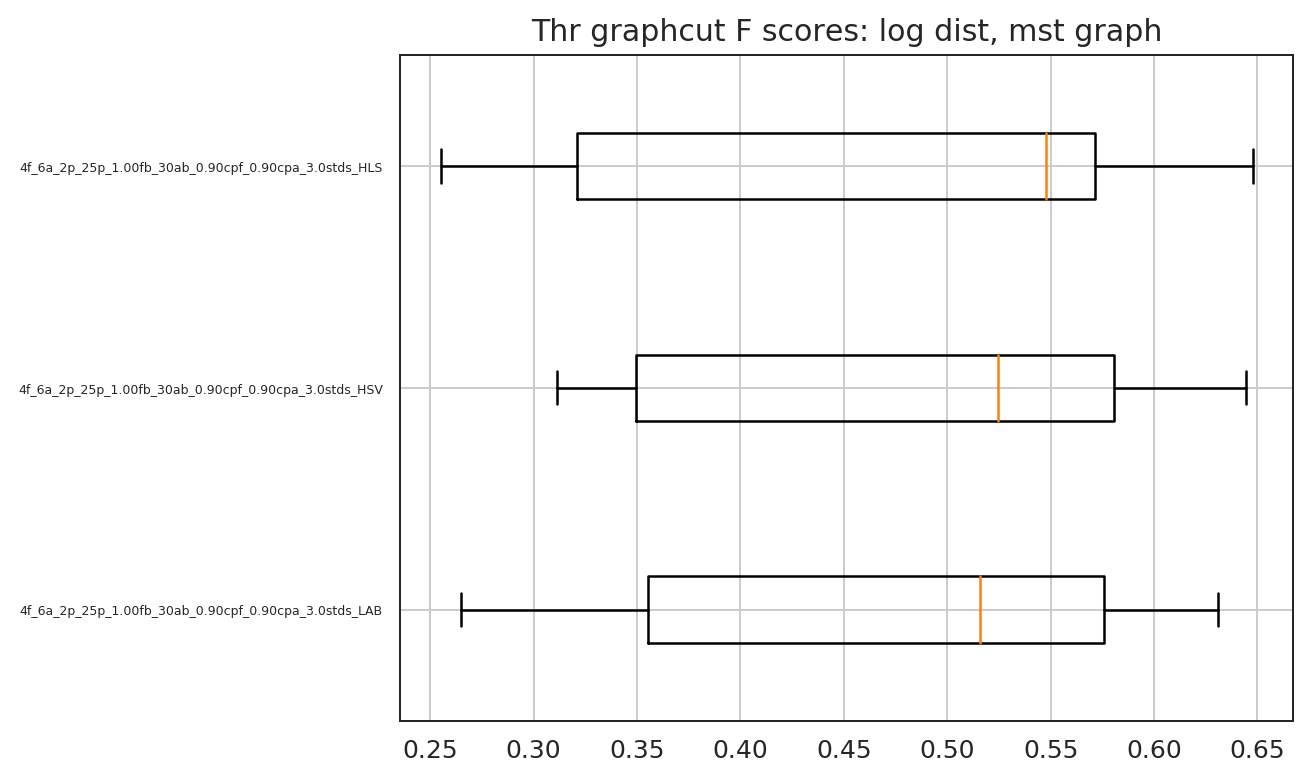
\includegraphics[width=\textwidth]{Thr_graphcut_Fscores_log_mst_boxplot.png} \\
%Scores using the sum of the computed gradients and the Threshold graph cut method\\
%\includegraphics[width=\textwidth]{Spectral_clustering_Fscores_global_complete_boxplot_pred_linreg.png} \\
%Scores using the gradients predicted by the linear regression model (LinReg) and the Spectral Clustering method\\
%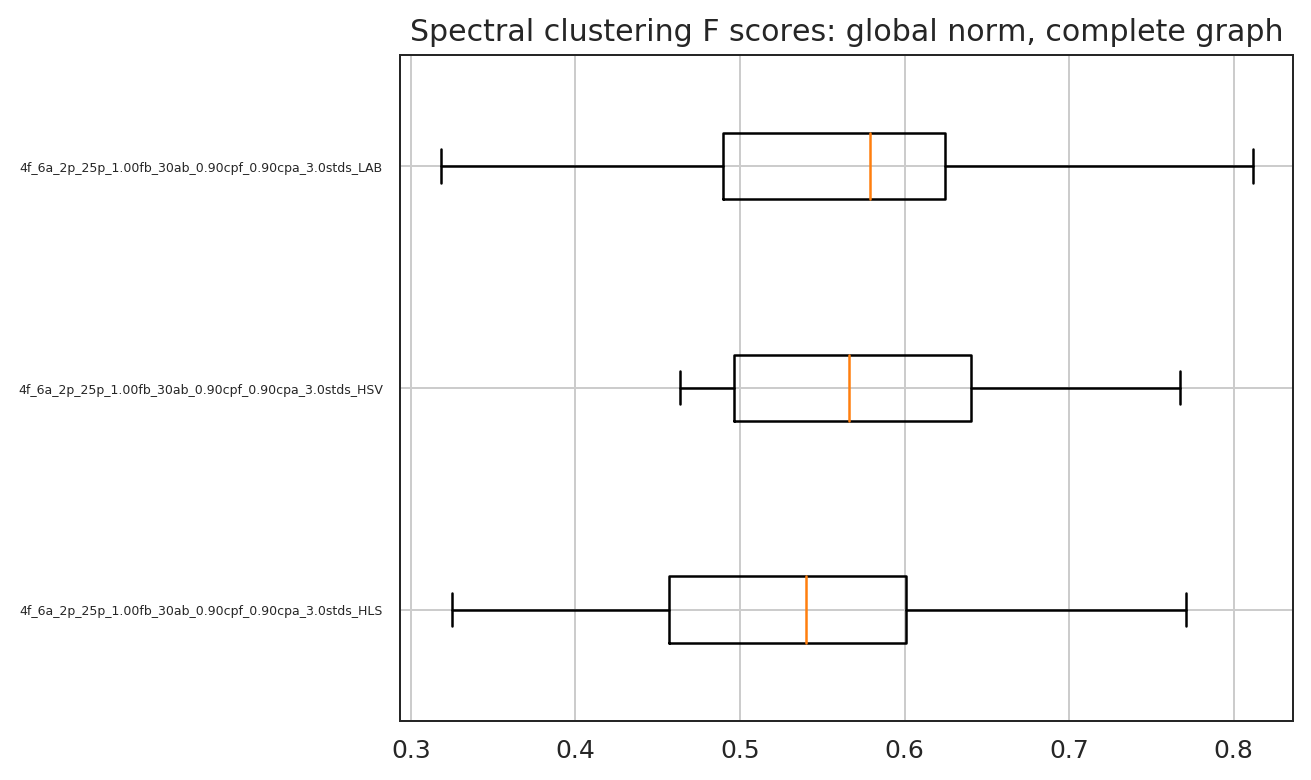
\includegraphics[width=\textwidth]{Spectral_clustering_Fscores_global_complete_boxplot.png}\\
%Scores using the sum of the computed gradients and the Spectral Clustering method\\

\section{Perceptual image segmentation}
\subsection{Hierarchical watershed}
\subsection{Interactive image segmentation}



\section{Comparison with the state of the art}
\subsection{Scores}

\begin{table}[]
\centering
\begin{tabular}{c|c|c|c||c|c|c|}
\cline{2-7}
                                  & \multicolumn{3}{c||}{\textbf{BSDS300}} & \multicolumn{3}{c|}{\textbf{BSDS500}} \\ \cline{2-7} 
                                  & ODS         & OIS        & AP         & ODS         & OIS        & AP         \\ \hline
\multicolumn{1}{|c|}{Human}       & 0.79        & 0.79       & -          & 0.80        & 0.80       & -          \\ \hline
\multicolumn{1}{|c|}{Ours}        & 0.65        & 0.67       & 0.62       & 0.66        & 0.68       & 0.62       \\
\multicolumn{1}{|c|}{Mean Shift}  & 0.63        & 0.66       & 0.54       & 0.64        & 0.68       & 0.56       \\
\multicolumn{1}{|c|}{Felz-Hutt}   & 0.58        & 0.62       & 0.53       & 0.61        & 0.64       & 0.56       \\
\multicolumn{1}{|c|}{NCuts}       & 0.62        & 0.66       & 0.43       & 0.64        & 0.68       & 0.45       \\
\multicolumn{1}{|c|}{Canny}       & 0.58        & 0.62       & 0.58       & 0.60        & 0.63       & 0.58       \\
\multicolumn{1}{|c|}{Pb}          & 0.65        & -          & -          & -           & -          & -          \\ \hline
\multicolumn{1}{|c|}{mPb}         & 0.67        & -          & -          & -           & -          & -          \\
\multicolumn{1}{|c|}{sPb}         & 0.68        & -          & -          & -           & -          & -          \\
\multicolumn{1}{|c|}{gPb}         & 0.70        & 0.72       & 0.66       & 0.71        & 0.74       & 0.65       \\
\multicolumn{1}{|c|}{gPb-owt-ucm} & 0.73        & 0.76       & 0.73       & 0.73        & 0.76       & 0.73       \\ \hline
\end{tabular}
\end{table}


\begin{table}[]
\centering
\begin{tabular}{c|c|c|c||c|c||c|c|}
\cline{2-8}
                                  & \multicolumn{7}{c|}{\textbf{BSDS500}}                                                                                       \\ \cline{2-8} 
                                  & \multicolumn{3}{c||}{Covering $(\uparrow)$} & \multicolumn{2}{c||}{PRI $(\uparrow)$} & \multicolumn{2}{c|}{VI $(\downarrow)$} \\ \cline{2-8} 
                                  & ODS          & OIS          & Best         & ODS               & OIS               & ODS                & OIS               \\ \hline
\multicolumn{1}{|c|}{Human}       & 0.72         & 0.72         & -            & 0.88              & 0.88              & 1.17               & 1.17              \\ \hline
\multicolumn{1}{|c|}{Ours}        & 0.56         & 0.60         & 0.67         & 0.81              & 0.83              & 1.79               & 1.57              \\ \hline
\multicolumn{1}{|c|}{gPb-owt-ucm} & 0.59         & 0.65         & 0.74         & 0.83              & 0.86              & 1.69               & 1.48              \\ \hline
\multicolumn{1}{|c|}{Mean Shift}  & 0.54         & 0.58         & 0.66         & 0.79              & 0.81              & 1.85               & 1.64              \\ \hline
\multicolumn{1}{|c|}{Felz-Hutt}   & 0.52         & 0.57         & 0.69         & 0.80              & 0.82              & 2.21               & 1.87              \\ \hline
\multicolumn{1}{|c|}{Ncuts}       & 0.45         & 0.53         & 0.67         & 0.78              & 0.80              & 2.23               & 1.89              \\ \hline
\end{tabular}
\end{table}

\begin{figure}[!ht]
	\centering
	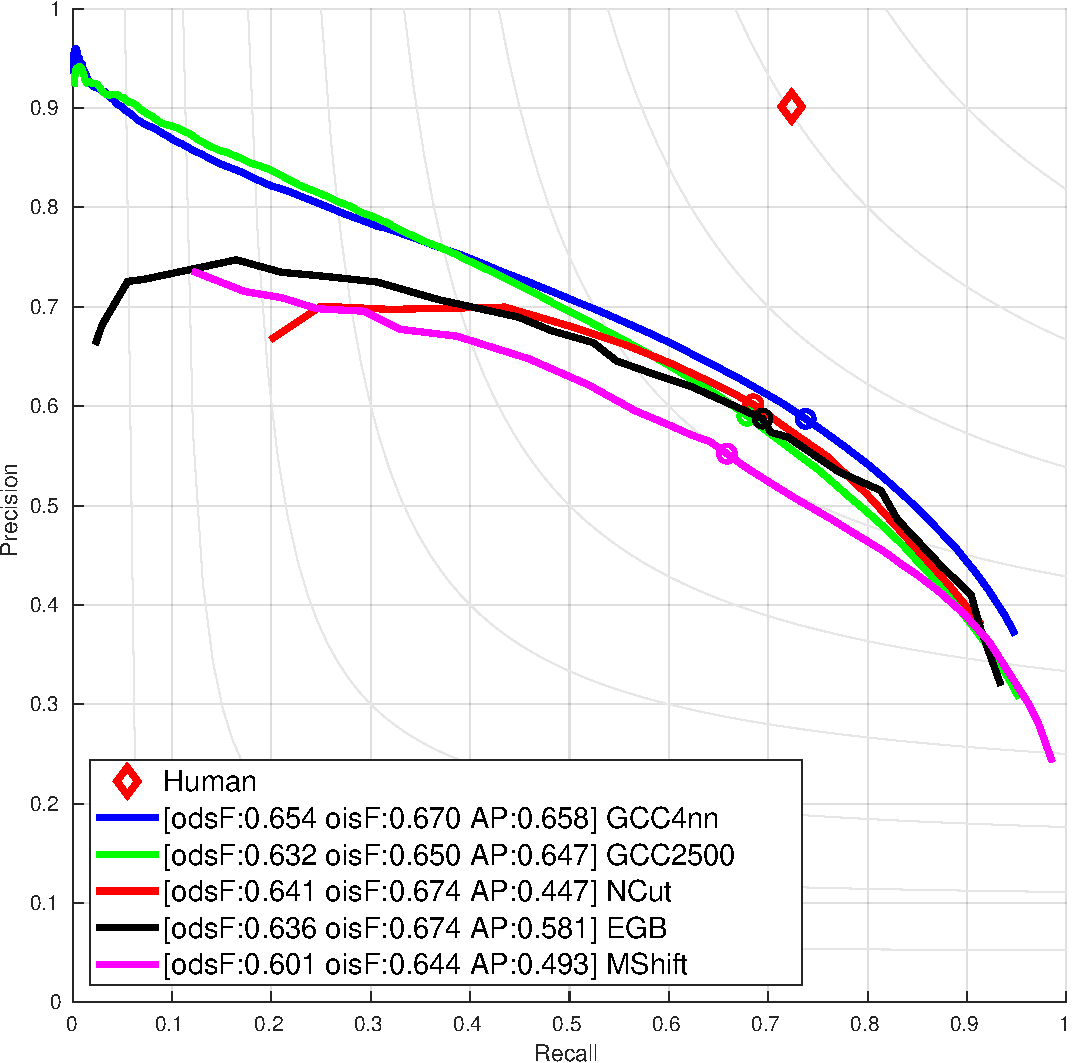
\includegraphics[width=\textwidth]{pr_curves_mymethod}
	\caption{Precision-recall plot of different contour detectors.}\label{fig:pipeline_gabor_image_segmentation}
\end{figure}
\subsection{Results}


\section{Importance of color and texture in image segmentation}


\section{Conclusions}
